\documentclass[a4paper]{report}
\usepackage[utf8]{inputenc}
\usepackage[T1]{fontenc}
\usepackage{RJournal}
\usepackage{amsmath,amssymb,array}
\usepackage{booktabs}
\usepackage{hyperref}

\usepackage{Sweave}
\begin{document}

%% do not edit, for illustration only
\sectionhead{Contributed research article}
\volume{XX}
\volnumber{YY}
\year{20ZZ}
\month{AAAA}

%% replace RJtemplate with your article
\begin{article}
\Sconcordance{concordance:ephmetrics.tex:ephmetrics.rnw:%
1 8 1 1 0 20 1 1 6 13 1 1 2 1 0 1 1 16 0 1 2 1 1 1 4 7 0 1 2 2 1 1 2 1 %
0 1 1 13 0 1 2 19 1}


\title{Ephmetrics}
\author{Ben Morton 19'}

\maketitle

%%\VignetteIndexEntry{Using the facage package}
%%\VignetteDepends{facage}


\abstract{The \pkg{ephmetrics} package analyzes Williams College Archived Course Catalogs in PDF form and reports specific data. This data includes information about the given year's tuition price, and size of the undergraduate classes}

\section{Introduction}
This package was designed for an internship project and I set out to develop an automated way of receiving certain metrics about Williams College and its student body over the years. An institution like Williams prides itself on its diversity and growth over time, and the data is organized in a way where this growth and geographical diversity can be easily analyzed in visualizations and dataframes.


\section{Data}
The information in this package retrieves data from the Registrar Office of Williams College Archived Course Catalogs. These catalogs are found in PDF form, and the pdftools package was used to read and convert the PDF’s into text. Using the 2009-2010 catalog as a test case, functions were developed to capture the relevant information from the given year.
The format of the catalog from each year is not exactly uniform, so the functions require updating based on the assumptions that were made. Examples of this are column layouts, what specific data follows what, and the overall formatting of each year’s information.

\section{Examples of Using the Data}
The tuition price of the years is retrieved and organized in a table where the linear increase in price is clearly shown. The rates of inflation do not align directly with the increase in tuition price each year. If the annual rates of inflation are applied to each respective year’s tuition price, the inflated price increase is less than the historical increase in price(http://www.inflation.eu/inflation-rates/united-states/historic-inflation/cpi-inflation-united-states.aspx).

\begin{Schunk}
\begin{Sinput}
> price_data <- ephmetrics::get_price_data()
> price_data
\end{Sinput}
\begin{Soutput}
   Tuition Year
1    46330 2014
2    44660 2013
3    42938 2012
4    41190 2011
5    39250 2010
6    37400 2009
7    35438 2008
8    33478 2007
9    31548 2006
10   29786 2005
\end{Soutput}
\end{Schunk}


\begin{Schunk}
\begin{Sinput}
> print(ggplot(price_data, aes(x = Year, y = Tuition)) +
+         geom_line() +
+         geom_point())
\end{Sinput}
\end{Schunk}
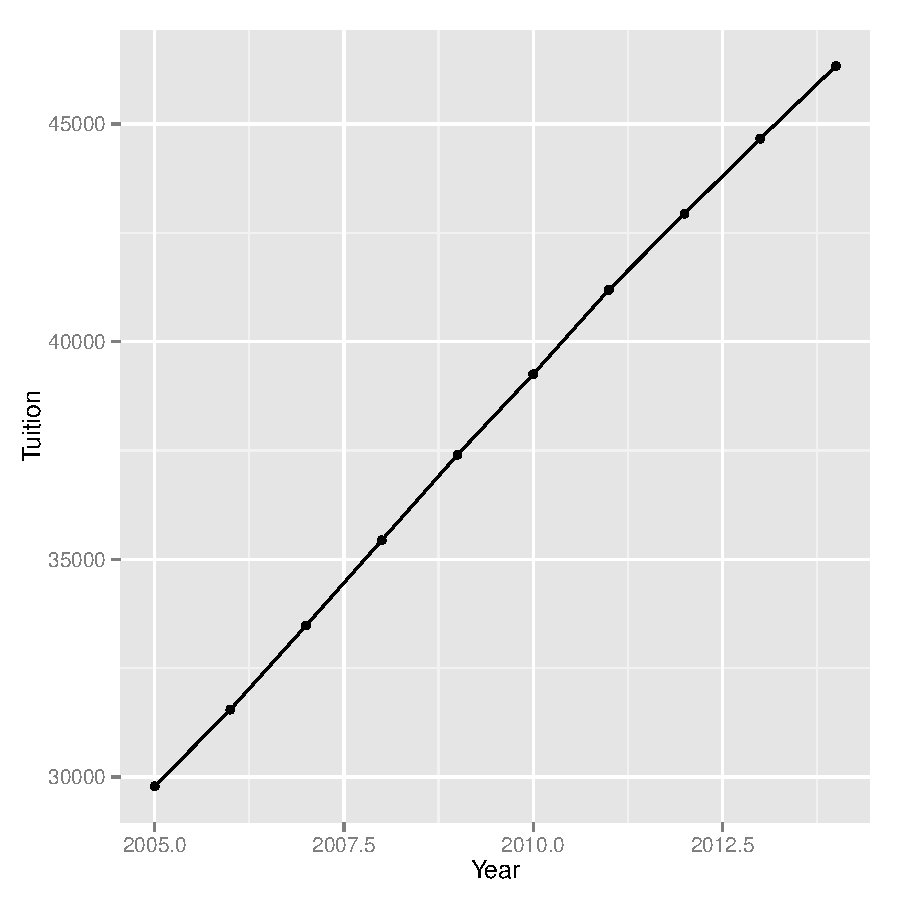
\includegraphics{ephmetrics-003}
\\The equation of the line is given as: y = 1861.1x - 4E+06. The slope and the low intercept shows that the tuition increases by fairly consistently by around 2000 dollars.\\\\
The package also includes a function to get enrollment data:

\begin{Schunk}
\begin{Sinput}
> enrollment_data <- ephmetrics::get_enrollment_data()
> enrollment_data
\end{Sinput}
\begin{Soutput}
  Year Freshmen Sophomores Juniors Seniors Graduate
1 2011      553        547     541     527       56
2 2010      541        548     533     515       48
3 2009      547        531     523     511       49
4 2008      538        533     522     531       46
5 2007      544        524     531     521       53
6 2006      534        532     529     506       59
7 2005      536        525     515     526       57
\end{Soutput}
\end{Schunk}
This enrollment data can be munged to analyze retention rates.

\section{Conclusion}
This package focuses on data grabbing and the information is presented in a clean r dataframe. This allows an interested subject to perform further analysis with the work.

The package ephmetrics is comprised of functions that aim to retrieve specific metrics about Williams College in a mechanical fashion. These functions collect and display data in a way that is easily understood by the reader and conclusions are able to be drawn from analyzing the results. Since the catalogs for different years are structured in slightly different ways, a way to improve this package would be to develop the functions in a way where the data could be more perfectly collected no matter the layout of the catalog.

\address{Ben Morton\\
  Mathematics and Computer Science\\
  Williams College\\
  Williamstown, MA, USA\\}
\email{bmm5@williams.edu}

\end{article}

\end{document}




